\documentclass{article}

% Language setting
% Replace `english' with e.g. `spanish' to change the document language
\usepackage[english]{babel}

% Set page size and margins
% Replace `letterpaper' with `a4paper' for UK/EU standard size
\usepackage[letterpaper,top=2cm,bottom=2cm,left=3cm,right=3cm,marginparwidth=1.75cm]{geometry}
\usepackage{algorithm}
\usepackage{algpseudocode}
\usepackage{amsmath}
\usepackage{graphicx}
\usepackage{booktabs}
\usepackage{pdflscape} % Add this package for landscape pages
\usepackage{caption,subcaption}
\usepackage[colorlinks=true, allcolors=blue]{hyperref}

\title{Image Analysis Assignment 4}
\author{Sherry Usman, Megan Mirnalini Sundaram R}
\begin{document}
\maketitle

\section*{Question 4.1}
\subsection*{Choice of Cells}
\par To pick a set of cells, pre-processing images to detect finer objects better is important. For that we first made the image single-channel by averaging the intensity values over all channels and creating a new gray-scale image. Then we applied morphological operations such as contrast stretching to remove underexposure areas and more accurately highlight the cells. Then we implemented an Opening operation to erode the objects(or foreground) and dilate it. This was done so that clusters of connected objects could be separated into separate distinct objects for better identification. Then a dilation operation was used to counteract the effects of erosion and to ensure that smaller objects did not completely disappear. Then, range thresholding was used to allow emphasis on areas of images with higher intensities (or cells). Lastly, labeling was used to give connected objects a unified symbol for better identification. Through this iterative procedure, we procured a series of images that were ready for image analysis.\newline 
\par For our series of images, we chose a set of points by implementing a function that randomly selected 15 rows from the rows of objects in the labeled images with the condition that the points were well within the data frame (between 50 and 450 in the x-axis and y-axis). Using the random points that were generated, we manually observed their behavior over the series of images and decided upon three criteria to keep/discard the points. 
\begin{itemize}
    \item how erratic their movement was
    \item whether they joined or merged with other cells
    \item whether or not they left the frame
\end{itemize}

Cells that were too erratic in their movements, merged or split from other cells, or left the frame were removed from our selection. This left us with a final set of cells that were more stable in their movement and did not leave the frame.

\begin{figure}[h!]
\centering
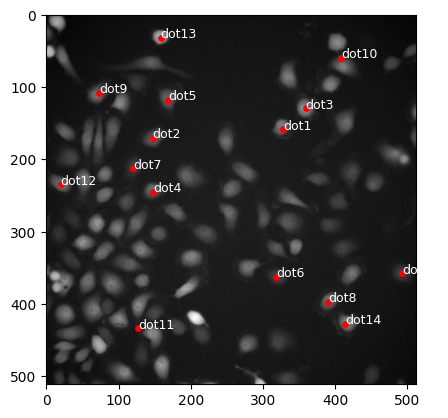
\includegraphics[width=0.75\linewidth]{Images/final_points_chosen.png}
\caption{\label{fig:ChoiceofCells-ControlSeries}The image shows the choice of cells in the \emph{Control Series}}
\end{figure}


\subsection*{Manual Check of the tracing of 5 cells}

We tracked the progress of 15 cells by creating an algorithm that iteratively finds the 15 closest objects/cells from the dataframe of the next image and then updates the objects' locations. This is done sequentially till image 30 and the result is a series of images with labeled cells. Our results are shown in Appendix 1. 

\subsection*{Algorithm to trace the cells}
To track the movement of the cells, the images must be processed first, to remove the glare and other distortions from the setup. Hence, the first part of the algorithm deals with the processing and labeling of the cells in the image. This allows us to gather further details on the cells, which were essential to tracing the cells. 

\begin{algorithm}[h!]
\caption{Tracing the Cells}\label{cell-trace}
\begin{algorithmic}[1]
\Procedure{TracingCells}{$\text{images}$}
    \State $\text{closest\_row[figure]} \gets \text{empty list}$
    \For{$\text{image}$ \textbf{in} $\text{images}$}
        \State $gray\_image \gets \text{Grayscale}(image)$
        \State $image\_contrasted \gets \text{ContrastStretch}(image)$
        \State $image\_eroded \gets \text{Erosion}(image\_contrasted)$
        \State $threshold\_image \gets \text{RangeThreshold}(mage\_eroded)$
        \State $image\_labeled \gets \text{Label}(threshold\_image)$
        \State Determine the center, size, and mean of each image
    \EndFor
    \State Compile the measurements into a dataframe
    \For{$\text{image}$ \textbf{in} $\text{images}$}
        \State $matching\_points \gets \text{center\_of\_gravity}(image) \And \text{center\_of\_gravity}(image+1)$
        \State $filtered\_matching\_points \gets \text{center\_of\_gravity}(image) \And \text{center\_of\_gravity}(image+1)$
        \State Superimpose points on images
    \EndFor
    \State \textbf{return} Graph of points on images
\EndProcedure
\end{algorithmic}
\end{algorithm}

\par The processing of the images is first done by converting the image to a grayscale, and then contrast stretching with a lower bound of 0 and an upper bound of 75. The contrast-stretched image was then subjected to erosion. This removed the white noise on the image and highlighted the cells of interest. The image was then, thresholded and labeled. This allowed us to get the measurements of the objects i.e., cells such as center of gravity, size and mean of the objects. 
\par The measurements were then compiled into a dataframe. The center of gravity of each object allowed us to track the movement in each image, as this served as the x- and y-coordinates for the movement. 
\subsection*{Application of Algorithm and Results}

\section*{Part 4.2}
\subsection*{Shape and Texture}


\begin{table}[h!]
\centering
\begin{tabular}{ |p{1.7cm}|p{1.7cm}|p{1.7cm}|p{1.7cm}|p{1.7cm}|p{1.7cm}|p{1.7cm}| }
\hline
\multicolumn{7}{|c|}{\textbf{Cell Features in A Series}} \\
\hline
\textbf{Models} & \textbf{Average Area} & \textbf{Perimeter} & \textbf{Roundness} & \textbf{Mean Intensity} & \textbf{Average Standard Deviation} & \textbf{Smoothness} \\
\hline
\textbf{Cell 1} & 681.38 & 8548.72 & 128.08 & 23481.72 & 681.38 & 0.99 \\
\textbf{Cell 2} & 953.28 & 8034.45 & 128.33 & 21312.41 & 953.31 & 0.99 \\
\textbf{Cell 3} & 965.24 & 7834.79 & 134.13 & 21193.45 & 965.76 & 0.99 \\
\textbf{Cell 4} & 887.34 & 8161.00 & 117.99 & 21281.72 & 887.34 & 0.99 \\
\textbf{Cell 5} & 871.72 & 6328.86 & 121.35 & 18226.55 & 872.00 & 0.99 \\
\textbf{Cell 6} & 1217.69 & 6137.69 & 166.84 & 17727.28 & 1218.03 & 0.99 \\
\textbf{Cell 7} & 1039.83 & 6217.72 & 143.28 & 17879.31 & 1040.03 & 0.99 \\
\textbf{Cell 8} & 1039.83 & 6217.72 & 143.28 & 17879.31 & 1040.03 & 0.99 \\
\textbf{Cell 9} & 2277.59 & 3895.48 & 227.32 & 15520.34 & 2305.00 & 0.99 \\
\textbf{Cell 10} & 5150.62 & 5740.38 & 485.59 & 17210.34 & 5312.45 & 0.99 \\
\textbf{Cell 11} & 747.55 & 3208.52 & 110.24 & 14301.38 & 748.83 & 0.99 \\
\textbf{Cell 12} & 635.62 & 4784.07 & 98.96 & 16984.14 & 635.62 & 0.99 \\
\textbf{Cell 13} & 750.14 & 5769.72 & 108.39 & 18252.76 & 750.24 & 0.99 \\
\textbf{Cell 14} & 732.97 & 7609.90 & 106.96 & 20932.76 & 733.03 & 0.99 \\
\textbf{Cell 15} & 387.24 & 3793.31 & 54.57 & 14664.62 & 387.38 & 0.99\\
\hline
\end{tabular}
\end{table}




\begin{table}[h!]
\centering
\begin{tabular}{ |p{1.7cm}|p{1.7cm}|p{1.7cm}|p{1.7cm}|p{1.7cm}|p{1.7cm}|p{1.7cm}| }
\hline
\multicolumn{7}{|c|}{\textbf{Cell Features in A Series}} \\
\hline
\textbf{Models} & \textbf{Average Area} & \textbf{Perimeter} & \textbf{Roundness} & \textbf{Mean Intensity} & \textbf{Average Standard Deviation} & \textbf{Smoothness} \\
\hline
\textbf{Cell 1} & 374.38 & 3103.83 & 128.08 & 13465.03 & 374.38 & 0.99 \\
\textbf{Cell 2} & 744.45 & 4224.79 & 125.90 & 15578.28 & 744.45 & 0.99 \\
\textbf{Cell 3} & 479.69 & 3046.28 & 89.84 & 13241.28 & 479.69 & 0.99 \\
\textbf{Cell 4} & 657.38 & 7416.93 & 110.84 & 18673.10 & 657.38 & 0.99 \\
\textbf{Cell 5} & 737.14 & 8457.34 & 120.98 & 19833.45 & 737.14 & 0.99 \\
\textbf{Cell 6} & 792.90 & 6694.55 & 127.98 & 17979.66 & 792.90 & 0.99 \\
\textbf{Cell 7} & 571.21 & 5840.88 & 100.84 & 17377.52 & 571.21 & 0.99 \\
\textbf{Cell 8} & 579.03 & 5803.84 & 100.74 & 17474.83 & 579.03 & 0.99 \\
\textbf{Cell 9} & 758.14 & 7444.23 & 127.70 & 19272.48 & 758.14 & 0.99 \\
\textbf{Cell 10} & 596.10 & 8074.52 & 106.17 & 20615.90 & 596.10 & 0.99 \\
\textbf{Cell 11} & 503.21 & 7720.45 & 91.83 & 20281.41 & 503.21 & 0.99 \\
\textbf{Cell 12} & 540.48 & 6665.48 & 97.17 & 19052.79 & 540.48 & 0.99 \\
\textbf{Cell 13} & 547.17 & 6202.03 & 95.64 & 18167.28 & 547.17 & 0.99 \\
\textbf{Cell 14} & 678.14 & 5711.48 & 113.63 & 17195.24 & 678.14 & 0.99 \\
\textbf{Cell 15} & 569.52 & 7338.17 & 89.87 & 20958.62 & 569.52 & 0.99 \\
\hline
\end{tabular}
\end{table}







\subsection*{Cell Velocity and Distance Trajectory}

\begin{landscape} % Begin the landscape environment
\begin{table}[htbp]
\centering
\caption{Velocity Changes for Cells in Series A }
\label{tab:velocity_changes}
\begin{tabular}{|l|c|c|c|c|c|c|c|c|c|c|c|c|c|c|c|}
\hline
 & \textbf{Cell 1} & \textbf{Cell 2} & \textbf{Cell 3} & \textbf{Cell 4} & \textbf{Cell 5} & \textbf{Cell 6} & \textbf{Cell 7} & \textbf{Cell 8} & \textbf{Cell 9} & \textbf{Cell 10} & \textbf{Cell 11} & \textbf{Cell 12} & \textbf{Cell 13} & \textbf{Cell 14} & \textbf{Cell 15} \\
\hline
\textbf{Change 1} & 1.5 & 2.0 & 1.8 & 1.6 & 2.1 & 1.3 & 2.4 & 1.7 & 2.2 & 1.8 & 2.5 & 1.9 \\
\hline
\textbf{Change 2} & 2.3 & 1.7 & 1.9 & 1.5 & 2.0 & 2.2 & 1.8 & 2.3 & 1.9 & 2.1 & 1.6 & 2.0 \\
\hline
\textbf{Change 3} & 1.8 & 1.5 & 2.2 & 1.7 & 1.6 & 2.0 & 1.9 & 2.1 & 1.8 & 2.2 & 1.7 & 1.8 \\
\hline
\textbf{Change 4} & 2.0 & 1.9 & 1.6 & 1.8 & 1.9 & 2.1 & 1.7 & 2.2 & 1.9 & 1.5 & 2.3 & 1.6 \\
\hline
\textbf{Change 5} & 1.2 & 2.1 & 1.5 & 2.0 & 1.7 & 2.3 & 1.8 & 2.4 & 1.6 & 2.0 & 1.9 & 1.7 \\
\hline
\end{tabular}
\end{table}
\end{landscape} % End the landscape environment}



\subsection*{Differences in Trajectory}
\subsection*{Differences in Conditions}
\subsection*{Correlation between speed with shape and texture}
\section*{Appendix 1}


\begin{figure}[h!]
\centering
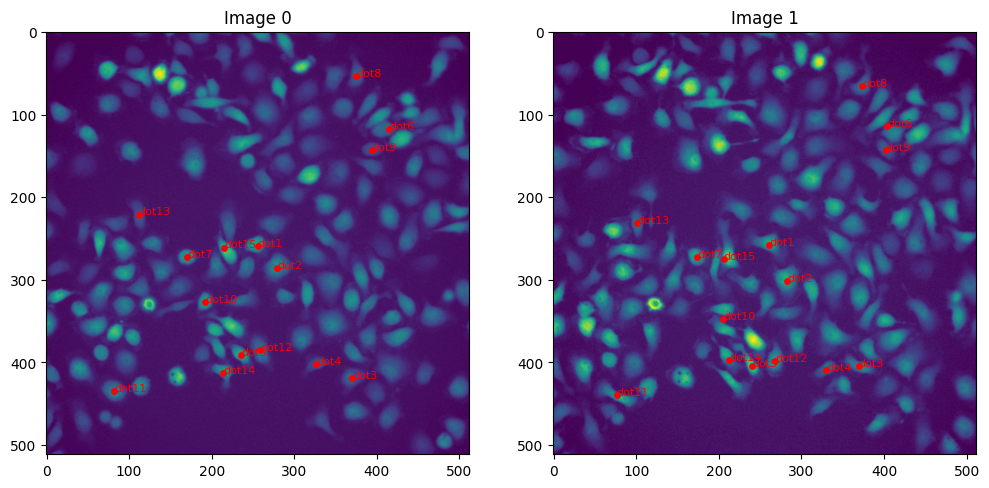
\includegraphics[width=0.75\linewidth]{Report/RImages/Traces_Growth/trace-b1.png}
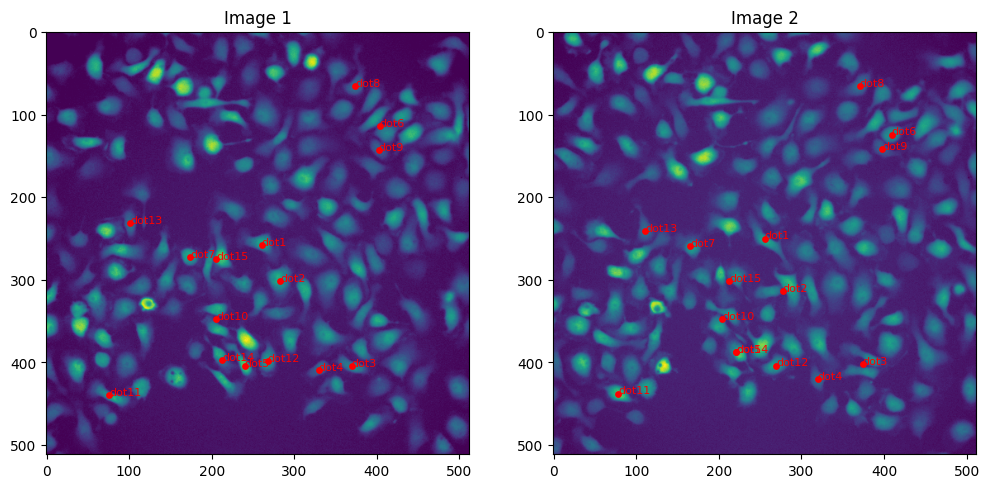
\includegraphics[width=0.75\linewidth]{Report/RImages/Traces_Growth/trace-b2.png}
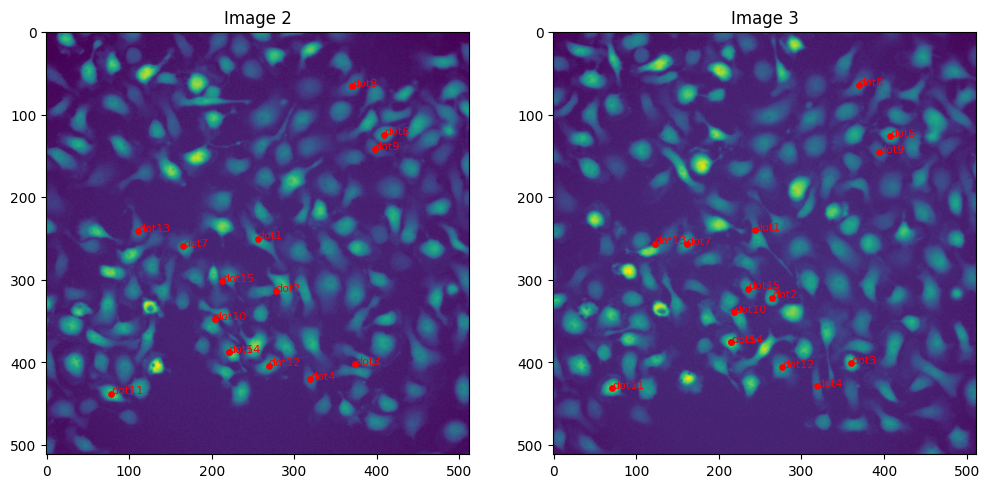
\includegraphics[width=0.75\linewidth]{Report/RImages/Traces_Growth/trace-b3.png}
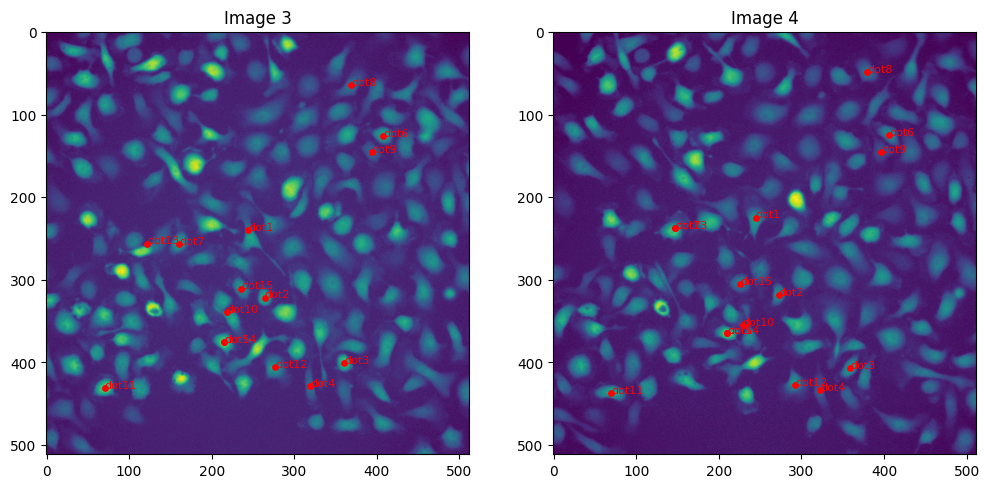
\includegraphics[width=0.75\linewidth]{Report/RImages/Traces_Growth/trace-b4.png}
\end{figure}

\clearpage

\begin{figure}[h!]
\centering
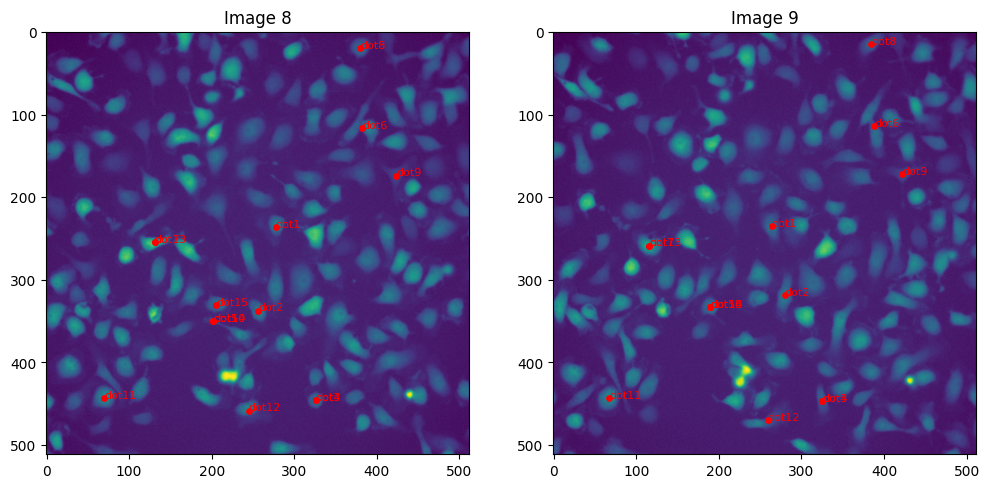
\includegraphics[width=0.75\linewidth]{Report/RImages/Traces_Growth/trace-b9.png}
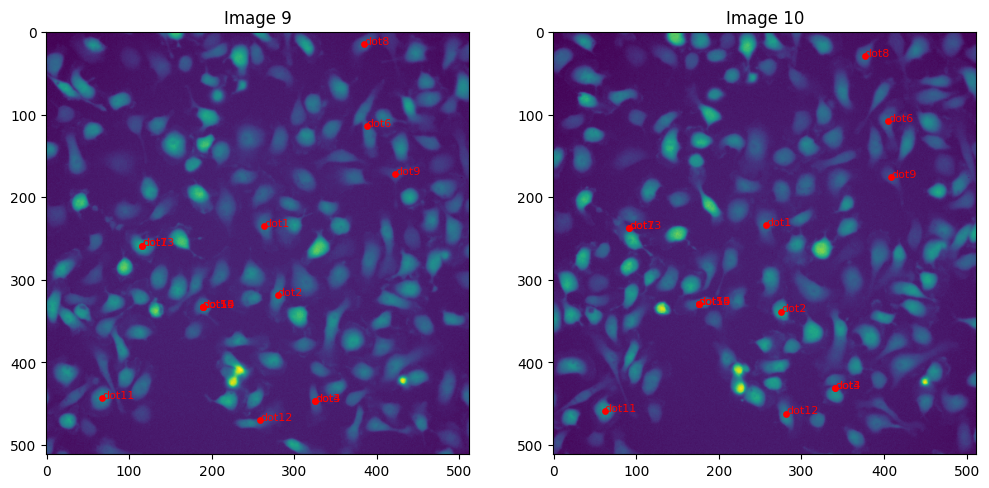
\includegraphics[width=0.75\linewidth]{Report/RImages/Traces_Growth/trace-b10.png}
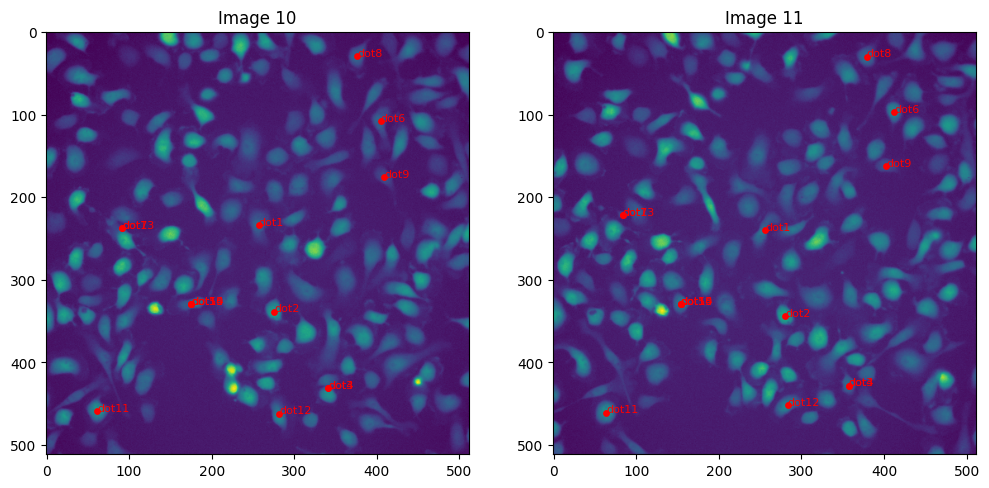
\includegraphics[width=0.75\linewidth]{Report/RImages/Traces_Growth/trace-b11.png}
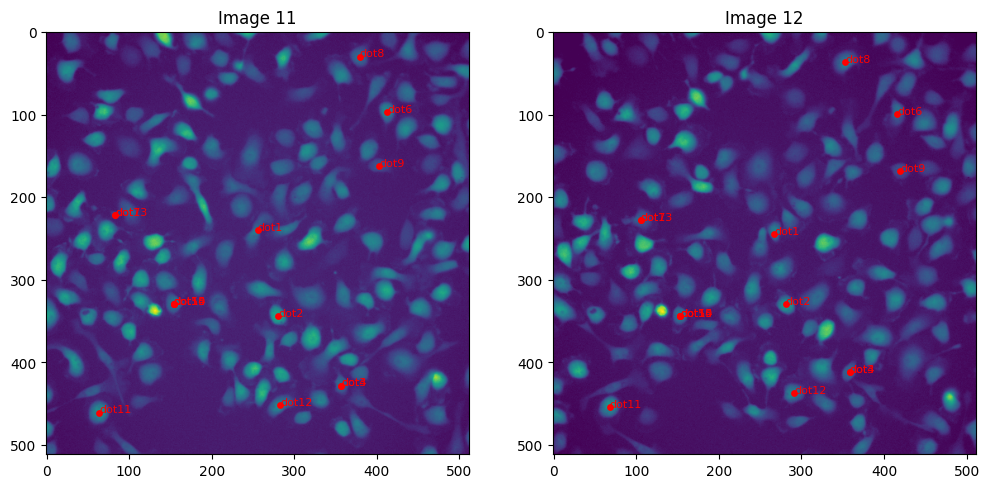
\includegraphics[width=0.75\linewidth]{Report/RImages/Traces_Growth/trace-b12.png}
\end{figure}

\clearpage

\begin{figure}[h!]
\centering
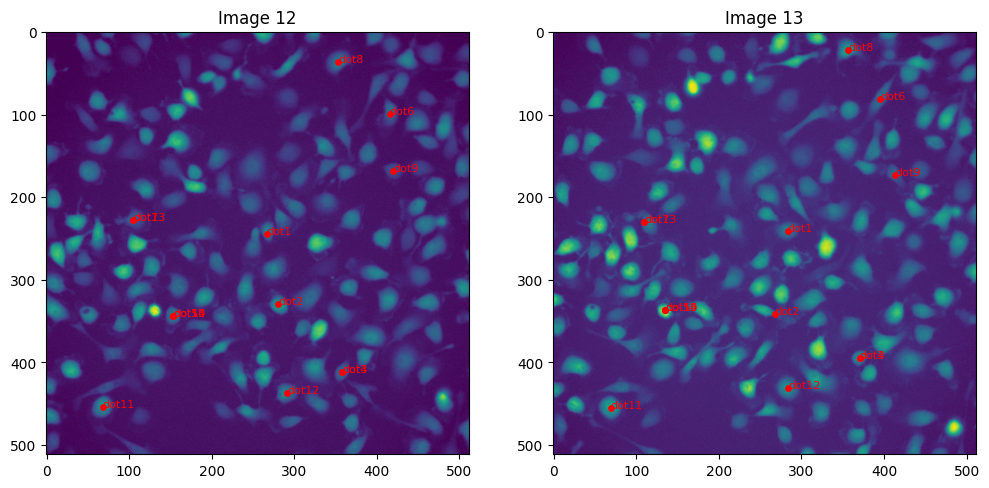
\includegraphics[width=0.75\linewidth]{Report/RImages/Traces_Growth/trace-b13.png}
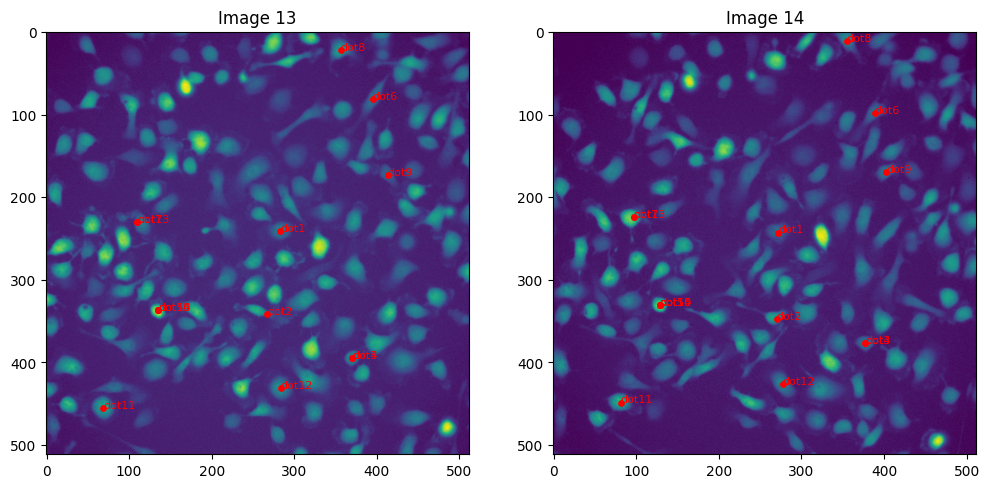
\includegraphics[width=0.75\linewidth]{Report/RImages/Traces_Growth/trace-b14.png}
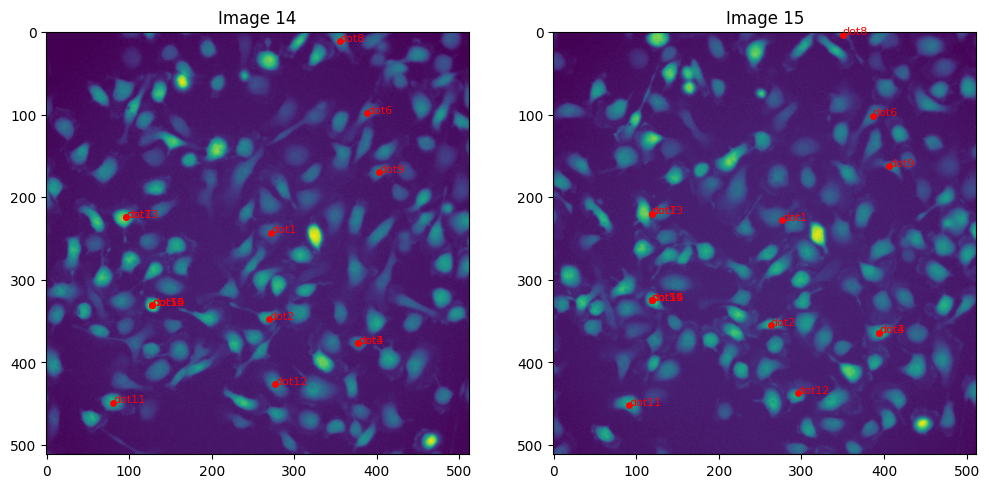
\includegraphics[width=0.75\linewidth]{Report/RImages/Traces_Growth/trace-b15.png}
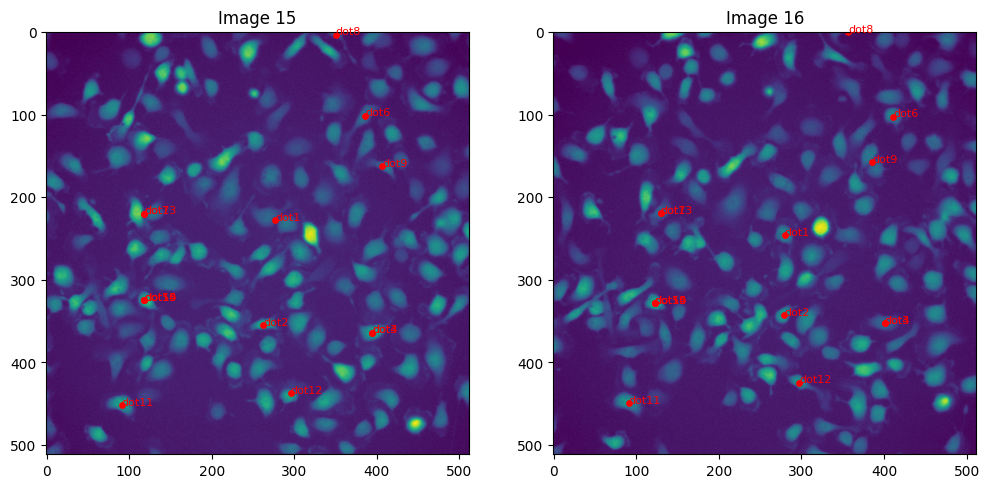
\includegraphics[width=0.75\linewidth]{Report/RImages/Traces_Growth/trace-b16.png}
\end{figure}

\clearpage

\begin{figure}[h!]
\centering
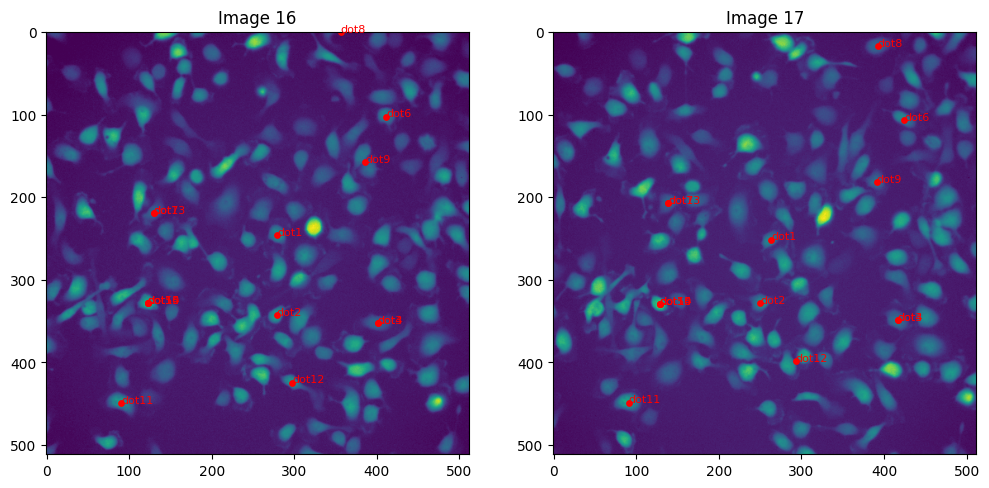
\includegraphics[width=0.75\linewidth]{Report/RImages/Traces_Growth/trace-b17.png}
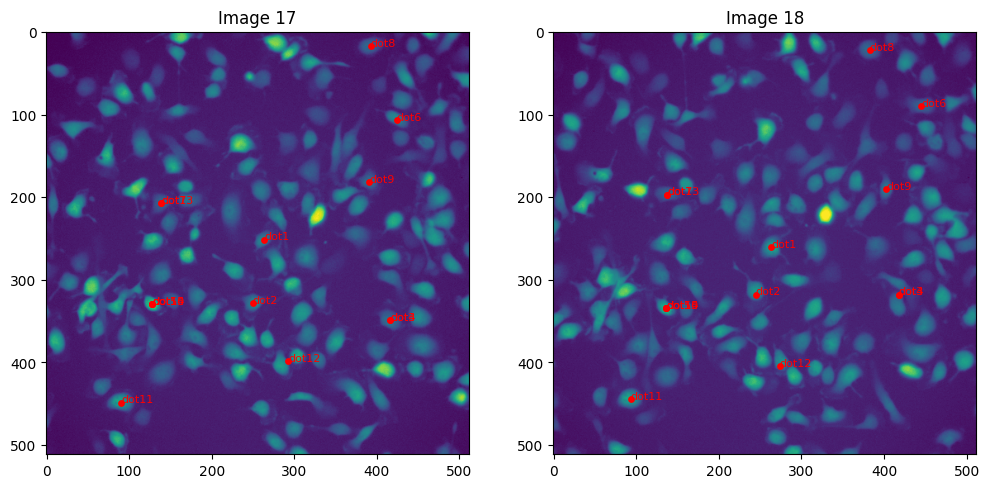
\includegraphics[width=0.75\linewidth]{Report/RImages/Traces_Growth/trace-b18.png}
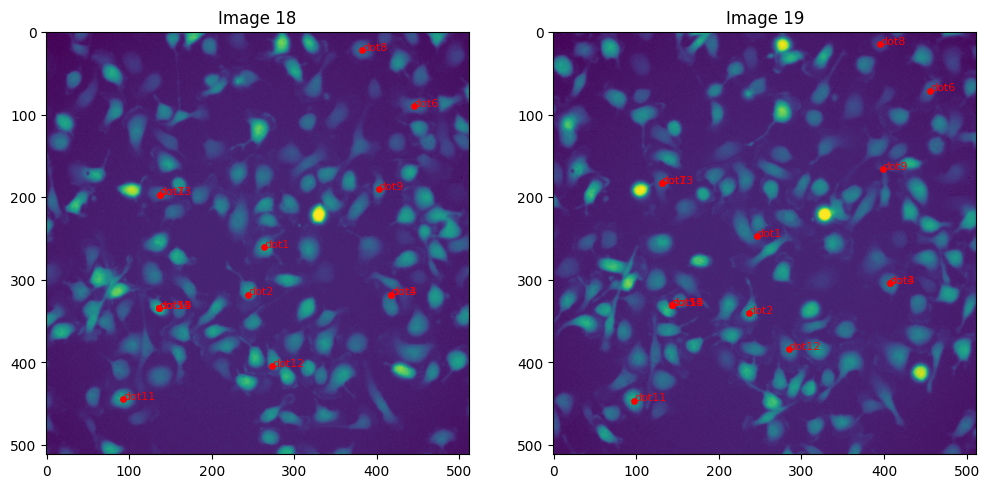
\includegraphics[width=0.75\linewidth]{Report/RImages/Traces_Growth/trace-b19.png}
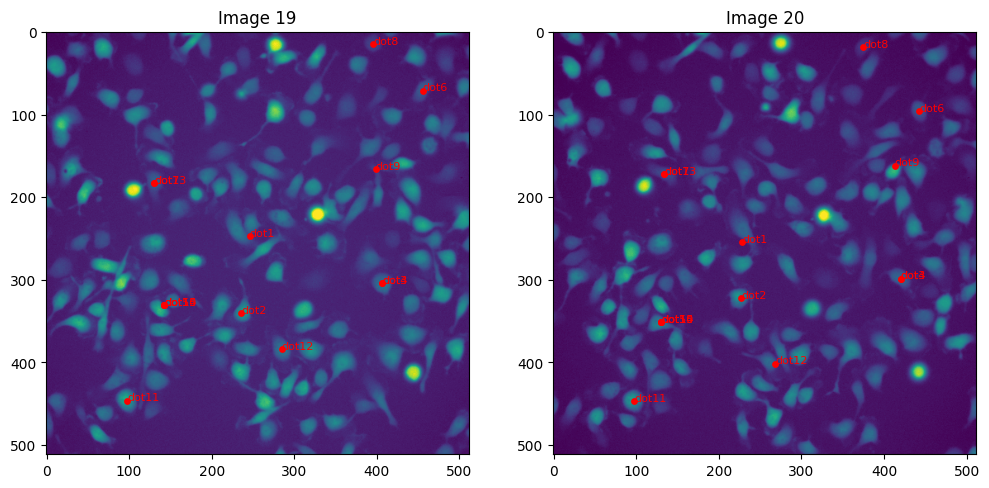
\includegraphics[width=0.75\linewidth]{Report/RImages/Traces_Growth/trace-b20.png}
\end{figure}

\clearpage

\begin{figure}[h!]
\centering
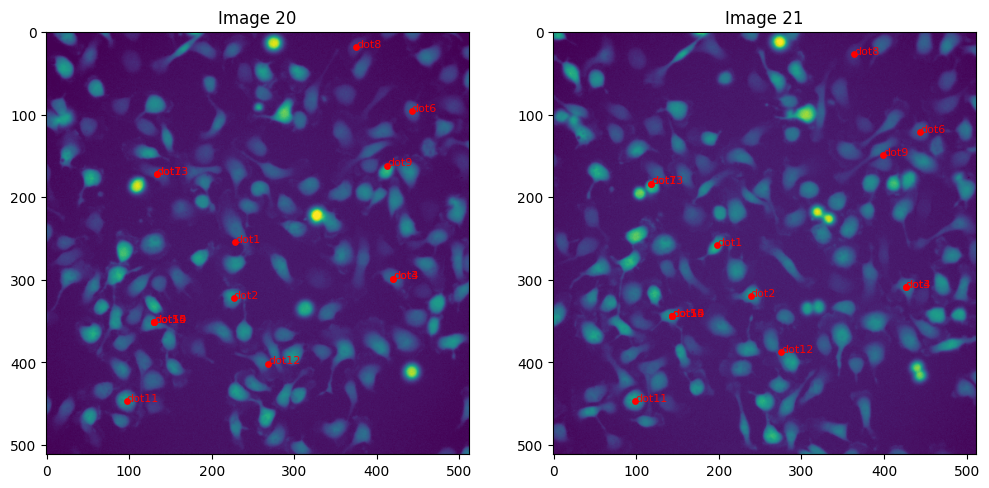
\includegraphics[width=0.75\linewidth]{Report/RImages/Traces_Growth/trace-b21.png}
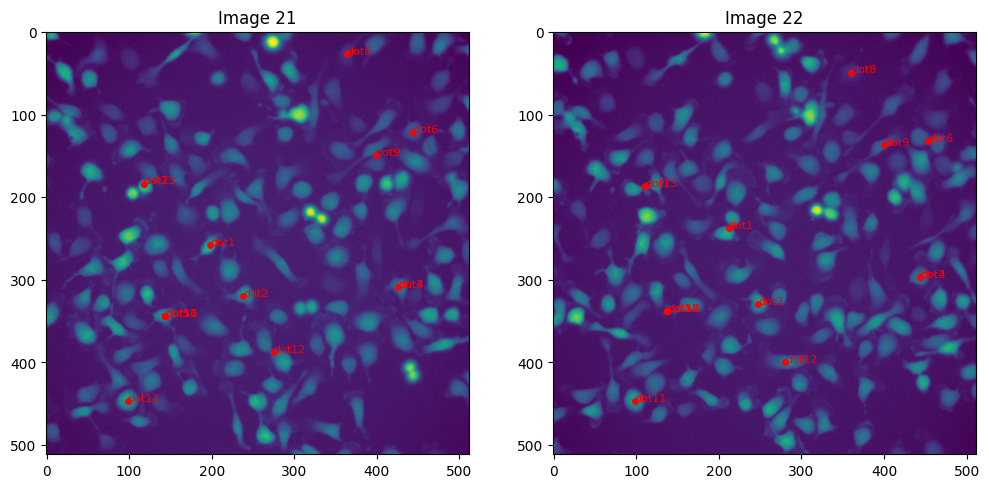
\includegraphics[width=0.75\linewidth]{Report/RImages/Traces_Growth/trace-b22.png}
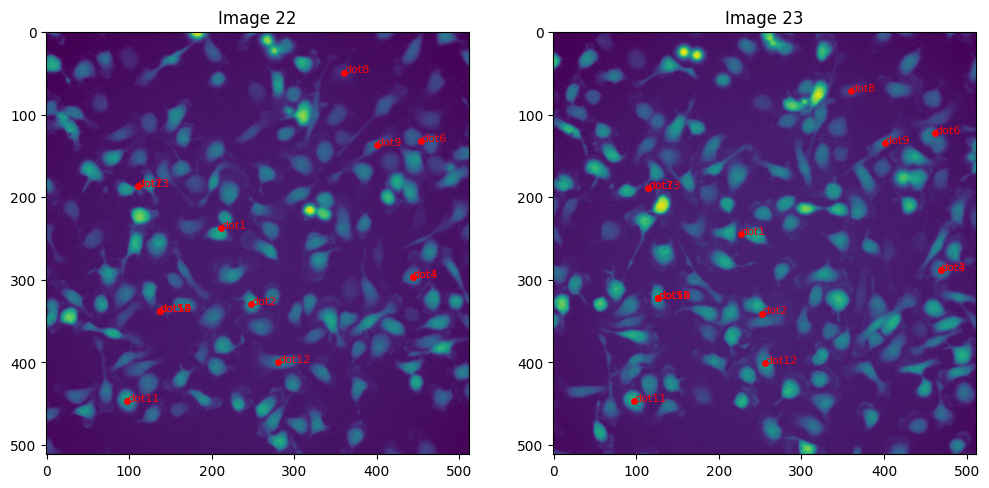
\includegraphics[width=0.75\linewidth]{Report/RImages/Traces_Growth/trace-b23.png}
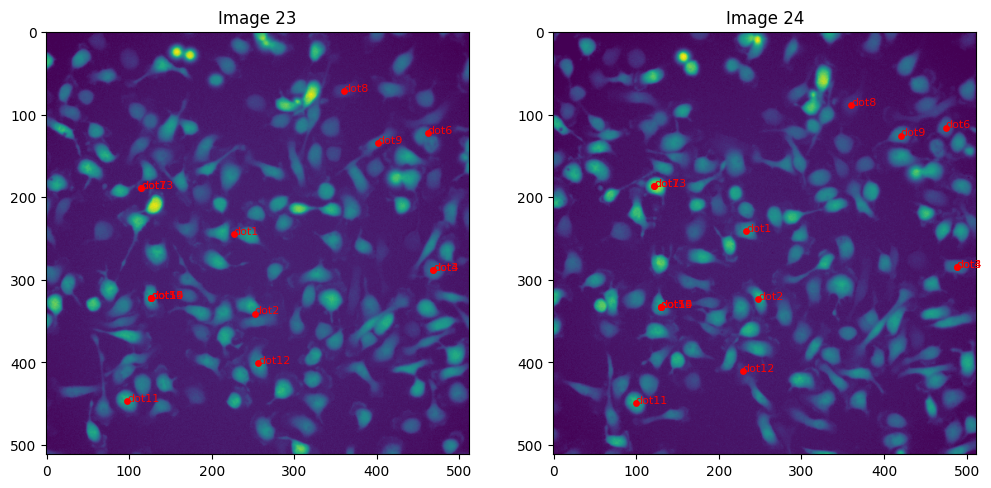
\includegraphics[width=0.75\linewidth]{Report/RImages/Traces_Growth/trace-b24.png}
\end{figure}

\clearpage

\begin{figure}[h!]
    \centering
    \begin{subfigure}[b]{0.5\linewidth}
        \centering
        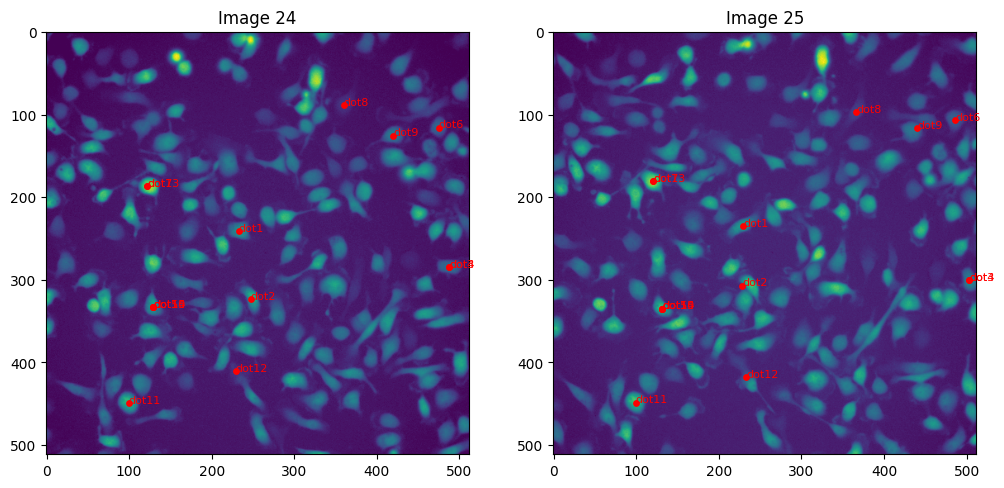
\includegraphics[width=\linewidth]{Report/RImages/Traces_Growth/trace-b25.png}
        \caption{}
    \end{subfigure}%
    \begin{subfigure}[b]{0.5\linewidth}
        \centering
        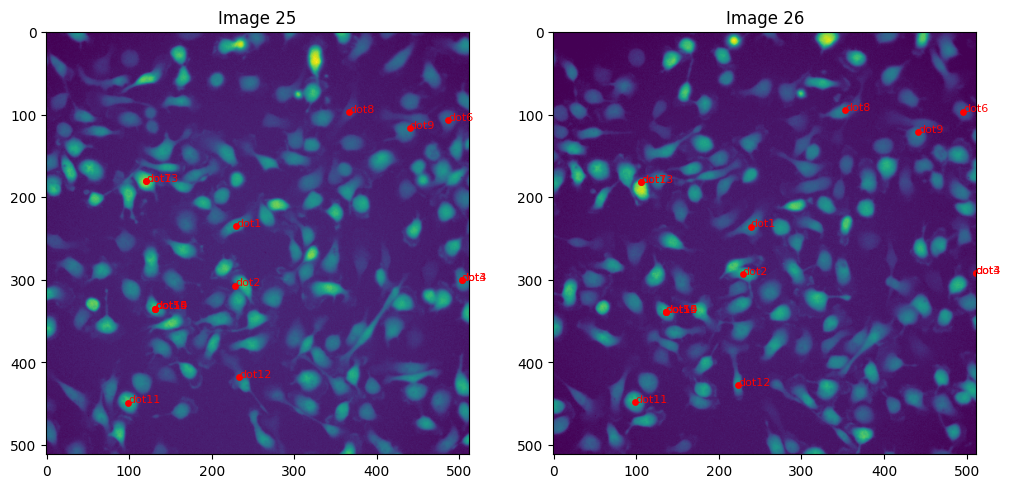
\includegraphics[width=\linewidth]{Report/RImages/Traces_Growth/trace-b26.png}
        \caption{}
    \end{subfigure}
    \begin{subfigure}[b]{0.5\linewidth}
        \centering
        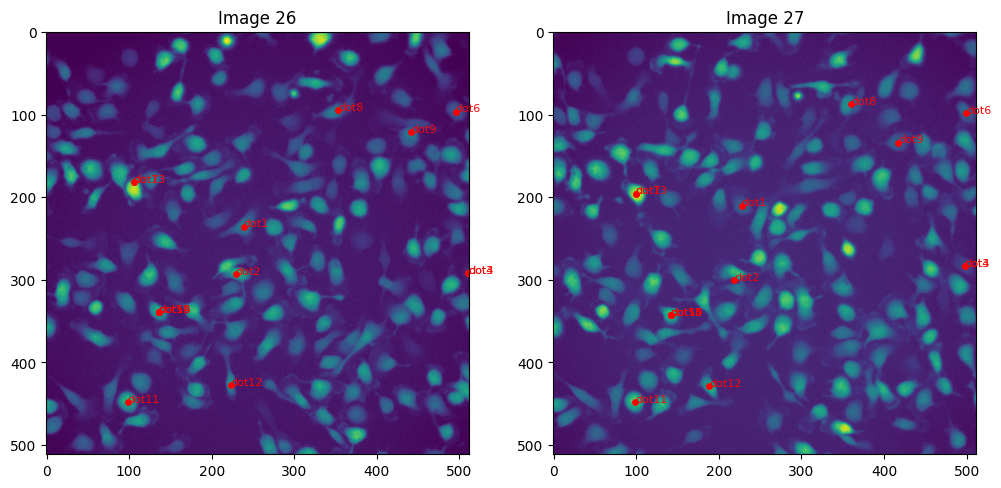
\includegraphics[width=\linewidth]{Report/RImages/Traces_Growth/trace-b27.png}
        \caption{}
    \end{subfigure}%
    \begin{subfigure}[b]{0.5\linewidth}
        \centering
        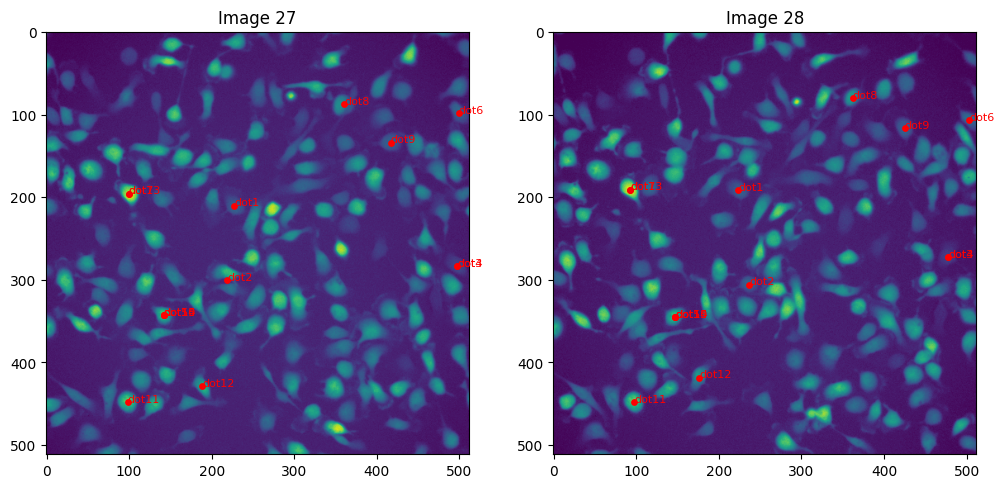
\includegraphics[width=\linewidth]{Report/RImages/Traces_Growth/trace-b28.png}
        \caption{}
    \end{subfigure}
    \caption{The image shows the choice of cells in the \emph{Control Series}}
    \label{fig:ChoiceofCells-ControlSeries}
\end{figure}

\newpage
\section*{Appendix 2}


\bibliographystyle{alpha}
\bibliography{sample}

\end{document}